\label{chapter-scenario-template}
\textbf{Created by:} Perawit Charoenwut \\
\textbf{Modified by:}

\subsection*{Scenario Objective}
This scenario aims to demonstrate how to model relationships between different types of agents in commercial transactions using the IOF Core patterns. The pattern models how different entities (such as persons and organizations) can take on specific roles (such as buyer and supplier) within complementary business processes that involve material products. This pattern is fundamental for representing any transaction where one party acquires a product from another, making it clear which agents are involved and what their specific roles are within the transaction context.

\subsection*{General Pattern Description}
The pattern models the relationship between buyers, suppliers, and material products through their roles and participation in business processes. It demonstrates how:

An agent classified as a Buyer has a BuyerRole that participates in a BuyingBusinessProcess
An agent classified as a Supplier has a SupplierRole that participates in a SupplyingBusinessProcess
Both business processes have the same MaterialProduct as a participant

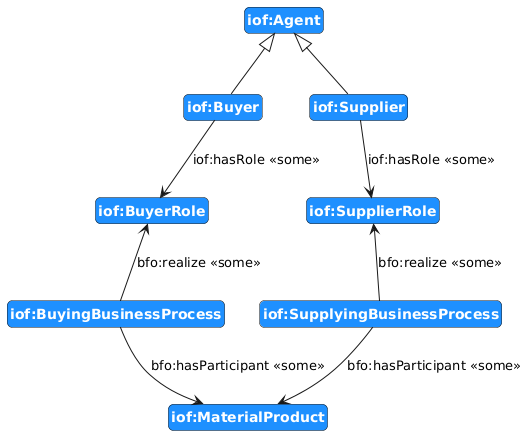
\includegraphics[scale=0.4]{scenarios/different-type-agent/image/different-type-agent-schema.png}

\subsection*{Use Case: Coffee Shop Transaction}
\subsubsection*{Use-Case Pattern Description}
This use case demonstrates how different types of agents (a person and an organization) participate in commercial transactions involving the purchase and supply of material products.

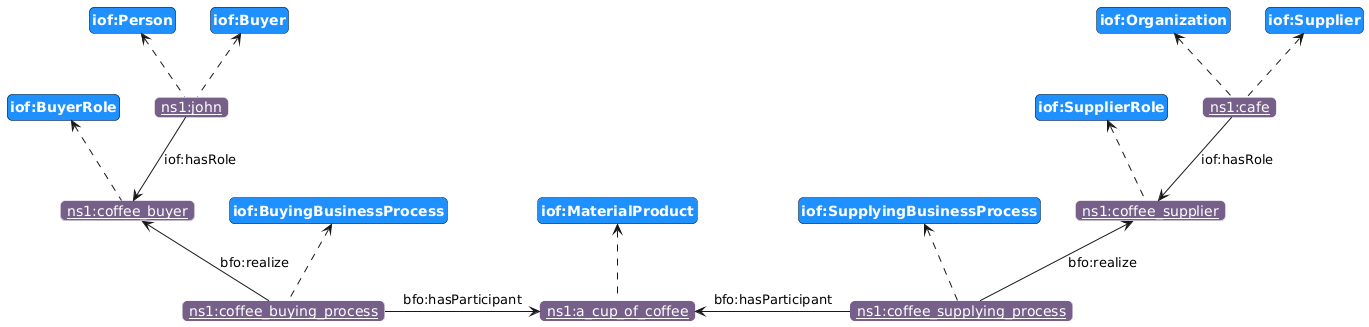
\includegraphics[scale=0.35]{scenarios/different-type-agent/image/different-type-agent.png}

\subsubsection*{Use-Case Example Data}
John (ns1:john) is both a person (iof:Person) and a buyer (iof:Buyer) of a cup of coffee (ns1:a-cup-of-coffee). John has a buyer role (ns1:coffe-buyer) which is bfo:realize through a buying business process (ns1:coffee-buying-process), where the cup of coffee participates (bfo:hasParticipant) in the buying process.

Simultaneously, a cafe (ns1:cafe) operates as both an organization (iof:Organization) and a supplier (iof:Supplier) with respect to the same cup of coffee (ns1:a-cup-coffee-cup). The coffee shop has a supplier role (ns1:coffee-supplier) which is bfo:realize through a supplying business process (ns1:coffee-supplying-process), where the same cup of coffee participates (bfo:hasParticipant) in the supplying process.

\begin{table}[h]
% \caption{}
\label{tab:organization-structure}
% \resizebox{\columnwidth}{!}{%
\begin{tabular}{|l|l|}
\hline

\hline
\end{tabular}%
% }
\end{table}


\subsubsection*{Data Mapping}
\begin{verbatim}
INSERT DATA {
    ns1:john a iof:Person, iof:Buyer ;
        iof:hasRole ns1:coffee-buyer.
    
    ns1:cafe a iof:Organization, iof:Supplier ;
        iof:hasRole ns1:coffee-supplier.
    
    ns1:coffee-buyer a iof:BuyerRole .
    
    ns1:coffee-supplier a iof:SupplierRole .
    
    ns1:coffee-buying-process a iof:BuyingBusinessProcess ;
        bfo:hasParticipant ns1:a-cup-of-coffee ;
        bfo:realize ns1:coffee-buyer .
    
    ns1:coffee-supplying-process a iof:SupplyingBusinessProcess ;
        bfo:hasParticipant ns1:a-cup-of-coffee ;
        bfo:realize ns1:coffee-supplier .
    
    ns1:a-cup-of-coffee a iof:MaterialProduct ;
\end{verbatim}



\subsubsection*{Data Validation}
\begin{verbatim}
#shape for Buyer
ns1:BuyerShape a sh:NodeShape ;
    sh:targetClass iof:Buyer ;
    sh:property [
        sh:path iof:hasRole ;
        sh:class iof:BuyerRole ;
        sh:minCount 1 ;
    ] ;
    sh:property [
        sh:path rdfs:subClassOf ;
        sh:hasValue iof:Agent ;
    ] .

# Shape for Supplier
ns1:SupplierShape a sh:NodeShape ;
    sh:targetClass iof:Supplier ;
    sh:property [
        sh:path iof:hasRole ;
        sh:class iof:SupplierRole ;
        sh:minCount 1 ;
    ] ;
    sh:property [
        sh:path rdfs:subClassOf ;
        sh:hasValue iof:Agent ;
    ] .

# Shape for BuyerRole
ns1:BuyerRoleShape a sh:NodeShape ;
    sh:targetClass iof:BuyerRole ;
    sh:property [
        sh:path [ sh:inversePath iof:hasRole ] ;
        sh:class iof:Buyer ;
        sh:minCount 1 ;
    ] .

# Shape for SupplierRole
ns1:SupplierRoleShape a sh:NodeShape ;
    sh:targetClass iof:SupplierRole .

# Shape for BuyingBusinessProcess
ns1:BuyingBusinessProcessShape a sh:NodeShape ;
    sh:targetClass iof:BuyingBusinessProcess ;
    sh:property [
        sh:path bfo:realize ;
        sh:class iof:BuyerRole ;
        sh:minCount 1 ;
    ] ;
    sh:property [
        sh:path bfo:hasParticipant ;
        sh:class iof:MaterialProduct ;
        sh:minCount 1 ;
    ] .

# Shape for SupplyingBusinessProcess
ns1:SupplyingBusinessProcessShape a sh:NodeShape ;
    sh:targetClass iof:SupplyingBusinessProcess ;
    sh:property [
        sh:path bfo:realize ;
        sh:class iof:SupplierRole ;
        sh:minCount 1 ;
    ] ;
    sh:property [
        sh:path bfo:hasParticipant ;
        sh:class iof:MaterialProduct ;
        sh:minCount 1 ;
    ] .

# Shape for MaterialProduct
ns1:MaterialProductShape a sh:NodeShape ;
    sh:targetClass iof:MaterialProduct .


\end{verbatim}